%%%%%%%%%%%%%%%%%%%%%%%%%%%%%%%%%%%%%%%%%%%%%%%%%%%%%%%%%%%%%%%%%%%%%%%%%%%%%%%%%
%%%%%                           EXPERIENCED MW                               %%%%
%%%%%%%%%%%%%%%%%%%%%%%%%%%%%%%%%%%%%%%%%%%%%%%%%%%%%%%%%%%%%%%%%%%%%%%%%%%%%%%%%

Thus far we have used the statutory minimum wage as our variable of interest. More 
precisely, we took the maximum across federal, state and local minimum wage as our 
treatment of interest. However, what matters for the a zipcode's housing market is 
the wage of the people residing there, which may not coincide with the statutory MW
if workers actually work in different zipcodes.

Therefore, we construct a new measure of the ``effective'' minimum wage in each zipcode 
that takes into account the fact that MW workers residence may differ from workplace 
location.

% Motivate experienced based on MW 


%%%%%%%%%%%%%%%%%%%%%%%%%%%%%%%%%%%%%%%%%%%%%%%%%%%%%%%%%%%%%%%%%%%%%%%%%%%%%%%%%
\subsection{A new minimum wage measure}

Following notation in section \autoref{sec:empirical_strategy}, we denote zipcodes by $i$
and monthly dates by $t$. Furthermore, for each zipcode $i$ define: (i) the set $\mathds{Z}_i$
of zipcodes in which residents of $i$ work (including $i$), and (ii) the set of weights 
$\{\omega_{iz}\}_{z \in \mathds{Z}_i}$ as 

\begin{equation*} \label{eq:weights}
	\omega_{iz} = \frac{N_{iz}}{N_i} ,
\end{equation*}
where $N_{iz}$ is the number of minimum wage workers who reside in zipcode $i$ and work in 
$z$, and $N_i$ is the total population of zipcode $i$. We define the experienced minimum 
wage measure as follows:

\begin{equation}
	\underline{w}^{\text{exp}}_{it} = \sum_{z \in \mathds{Z}_i} \omega_{iz} \underline{w}_{zt} \ 
	, \ \forall (i, t) . 
\end{equation}

The experienced MW of a zipcode is based on the minimum wages binding in other zipcodes where 
its residents work. An increase in a city, for example, may not have an impact in the local
rental market if most residents are not minimum wage workers. It will, however, affect 
neighboring zipcodes where MW workers reside. If what drives the effect is actually the supply
and demand of rental housing, then we would expect it to be larger. In practice, however, 
most MW changes arise from the state and thus our measures are highly correlated.

%% DESCRIBE HOW WE CONSTRUCT THE WEIGHTS

As an illustration, figure \ref{fig:expmw_san_diego} plots the statutory versus experienced 
MW variables following the California increase in the minimum wage on January, 2019. As of 
December 2018 the MW in San Diego city was \$11.50, whereas the state's MW binding outside 
the city was \$11.\footnote{For employers larger than 26 employees. For those below 26 
	employees the level was \$10.50.}
The increase in the state level MW to \$12 in January 2020 appears as a discontinuity in the 
city border. However, when we account for the fact that MW workers commute, we observe a 
gradient in the intensity of the policy.


\begin{figure}
	\caption{The California MW increase of January 2019 in San Diego}
	\label{fig:expmw_san_diego}
	\centering
	\begin{subfigure}[b]{0.55\textwidth}
		\caption{Statutory MW change}
		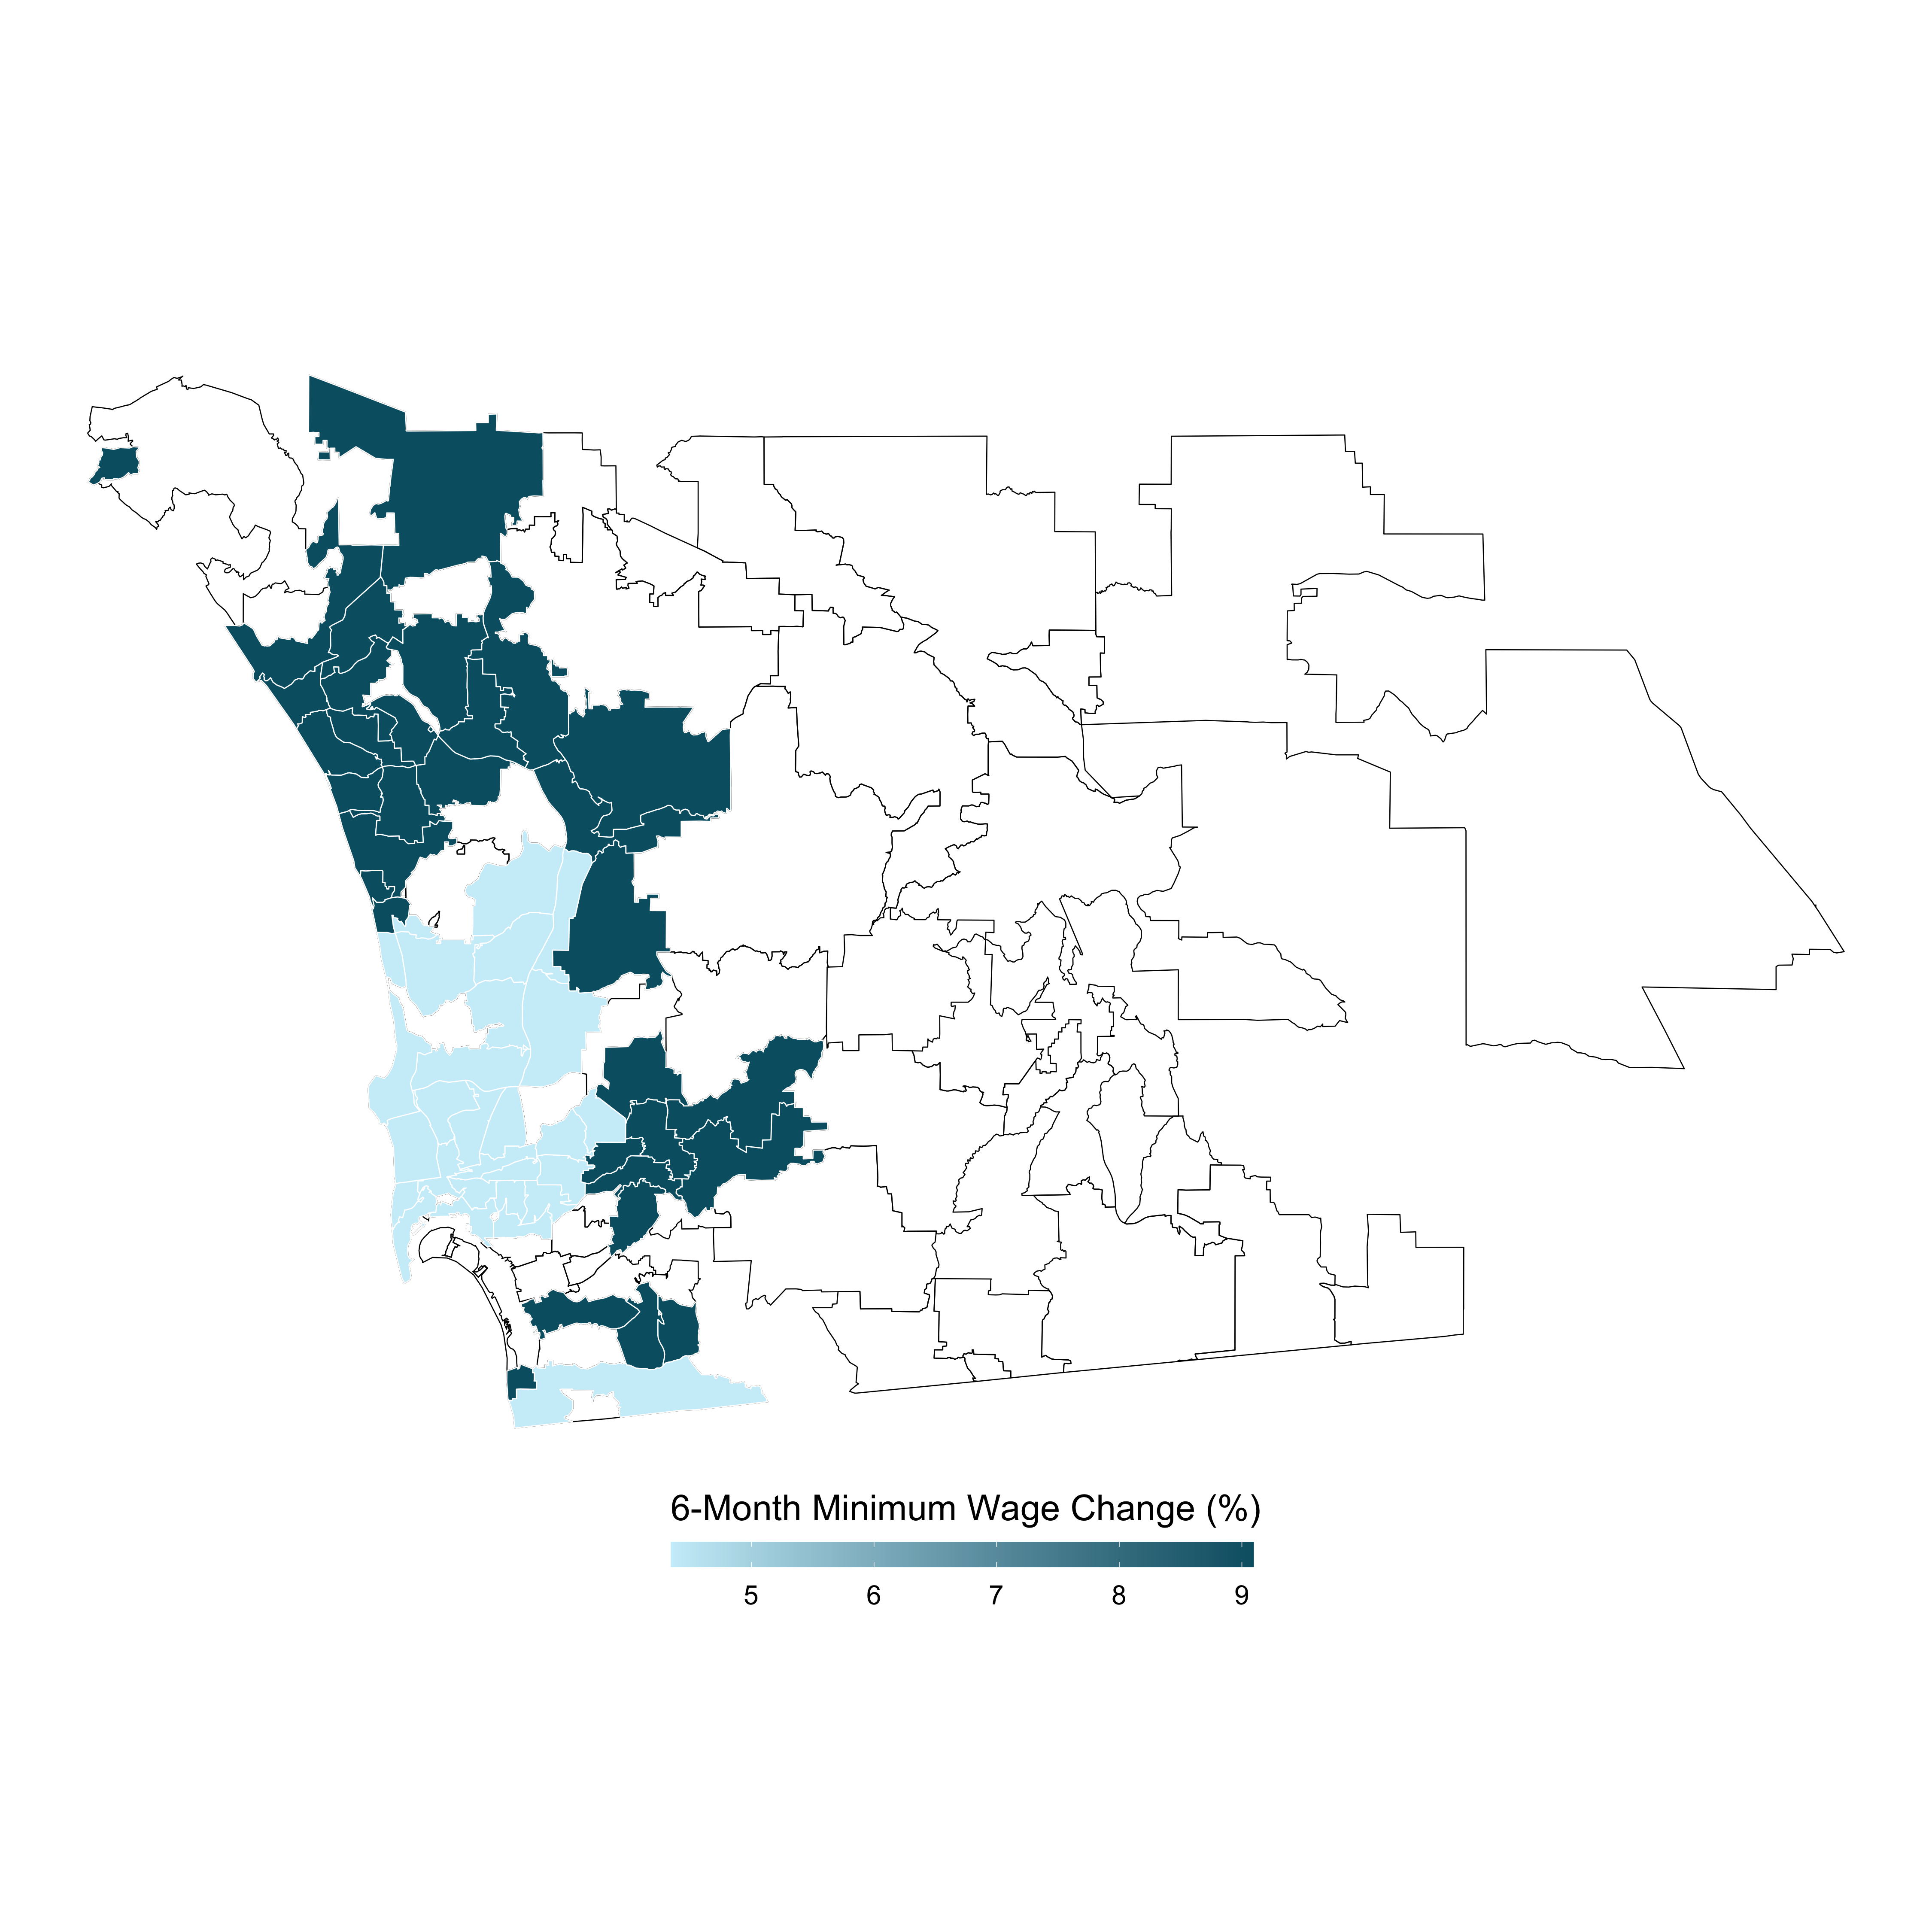
\includegraphics[width = \textwidth]
			{../../analysis/descriptive_maps/output/San_Diego_mw_msa.png}
	\end{subfigure}
	\begin{subfigure}[b]{0.55\textwidth}
		\caption{Experienced MW change}
		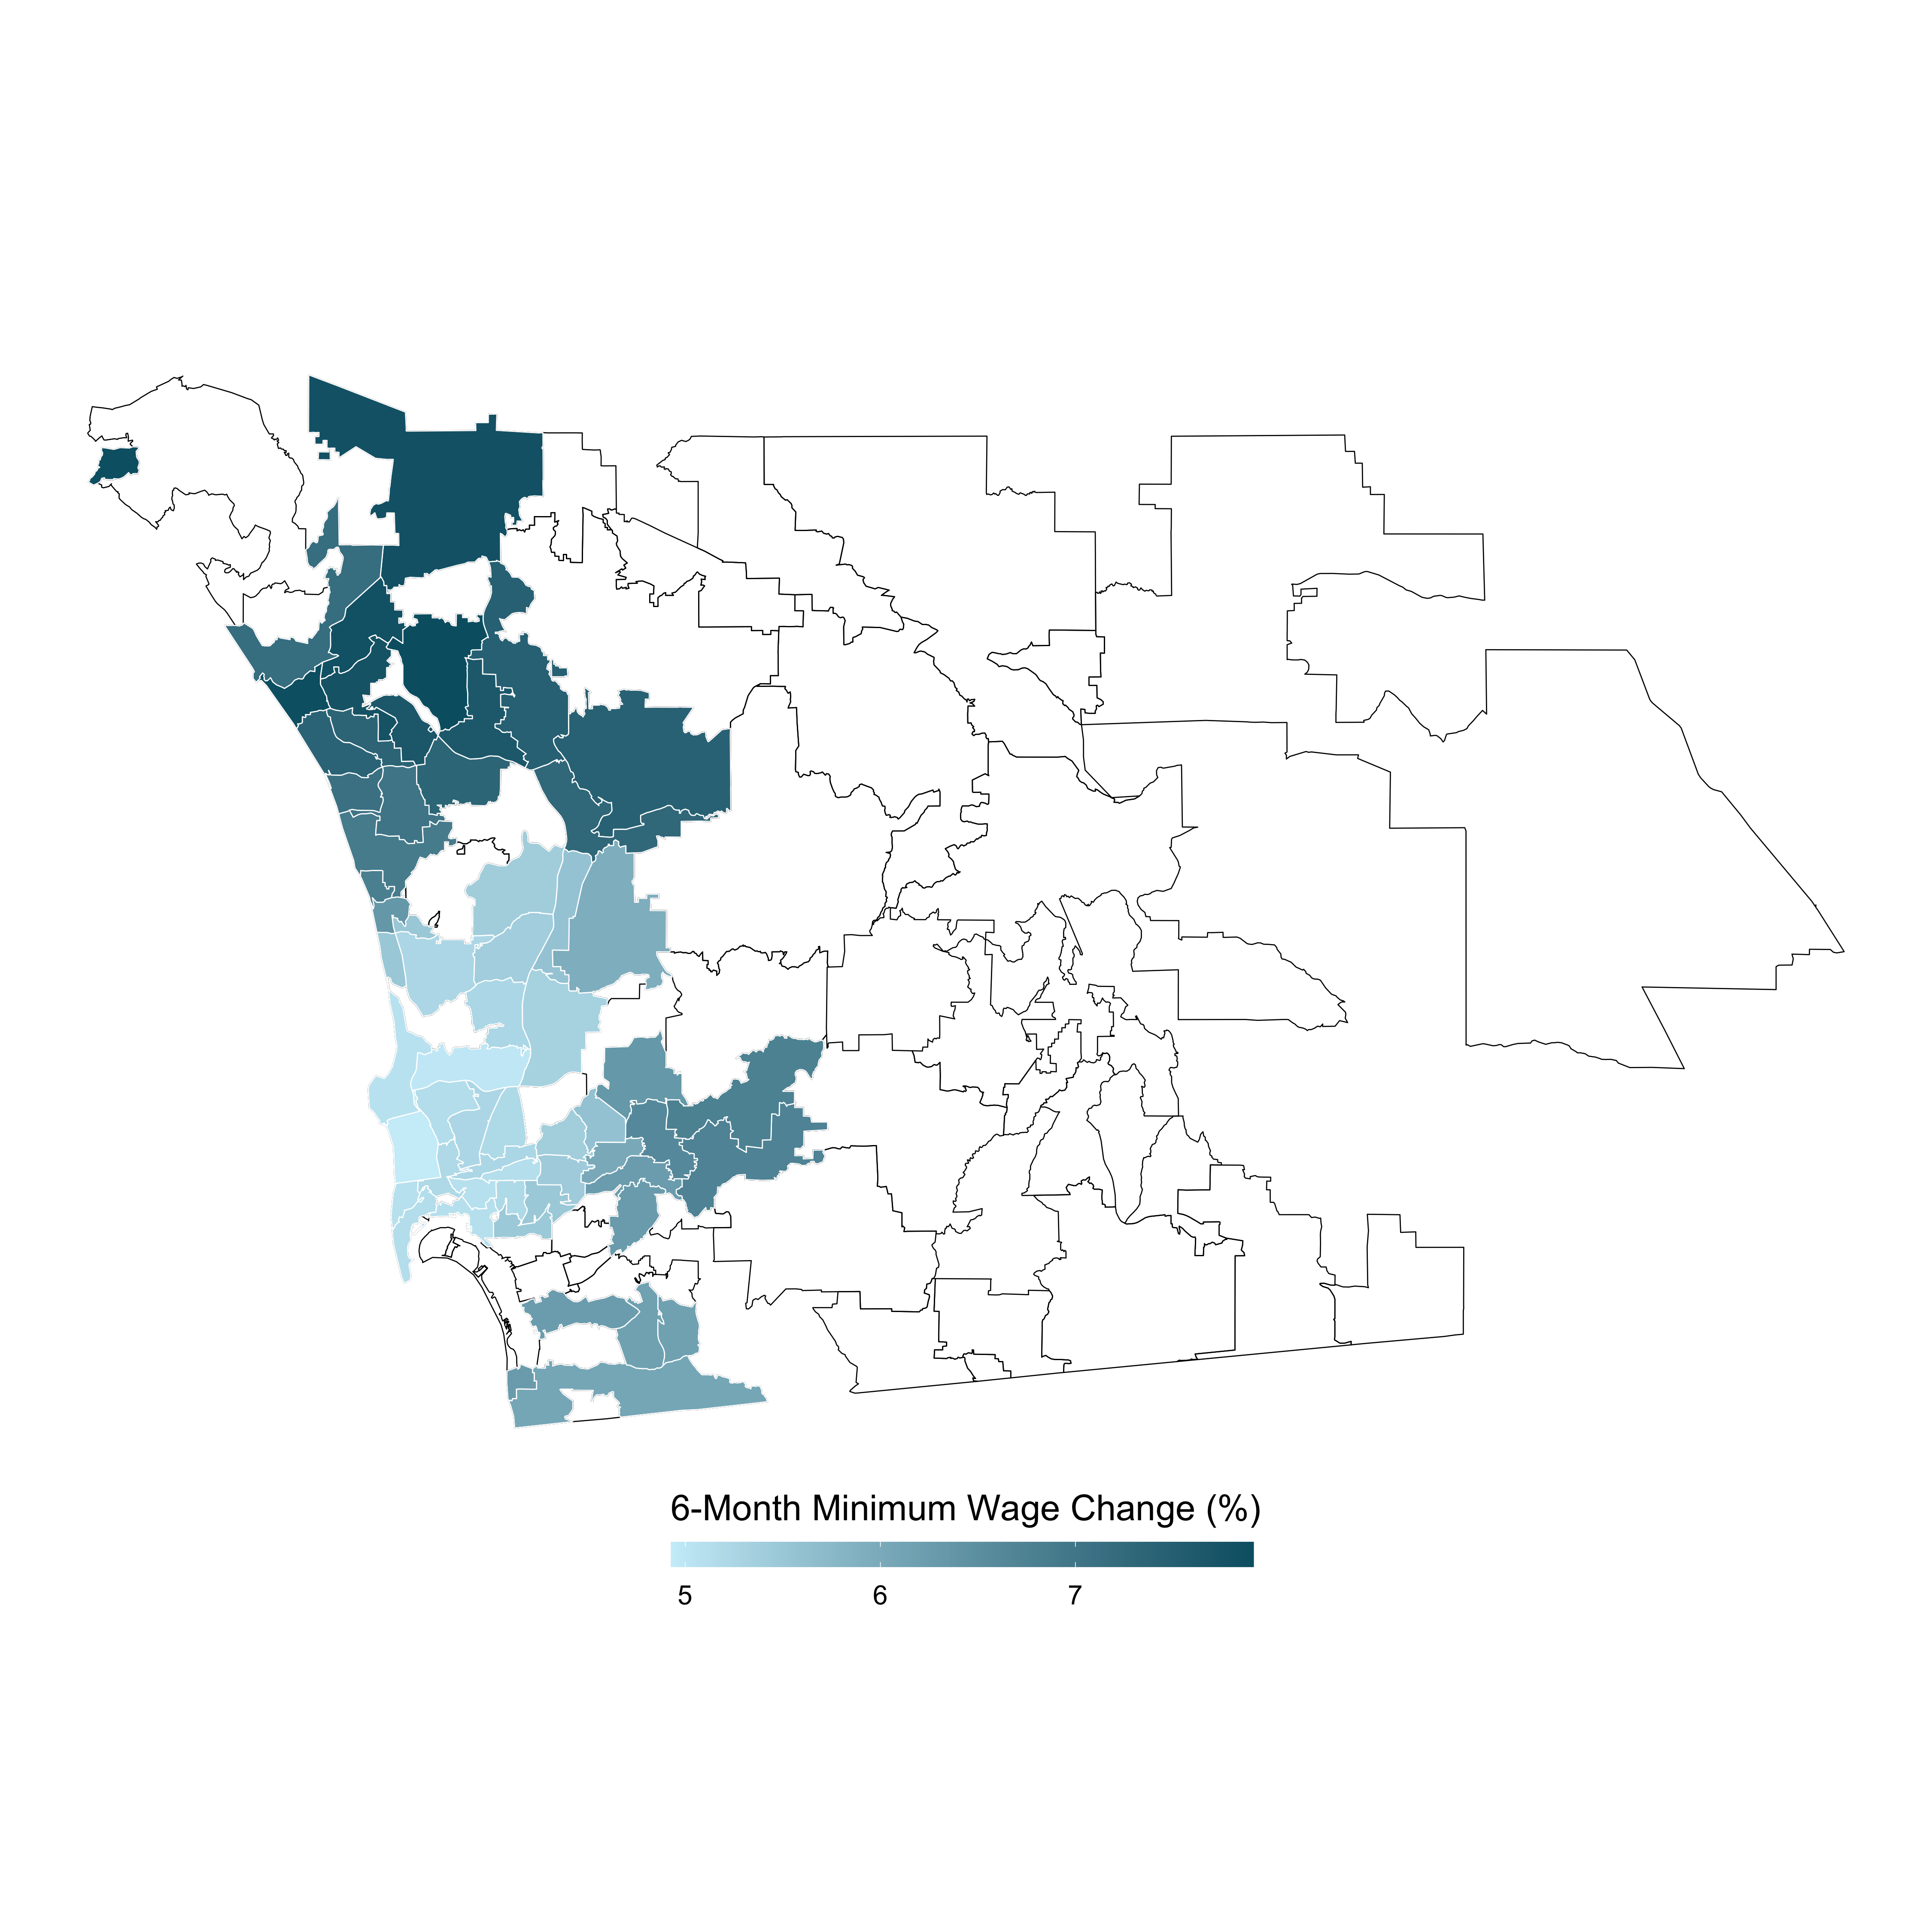
\includegraphics[width = \textwidth]
			{../../analysis/descriptive_maps/output/San_Diego_expmw_msa.png}
	\end{subfigure}
	\begin{minipage}{0.95\textwidth} \footnotesize
		\vspace{2mm} 
		\textit{Notes}: The figure maps the percent increase in our minimum wage and 
		experienced minimum wage measures following the state increase in California
		on January 2019. The map colors only zipcodes for which we have non-missing 
		rents data from Zillow.
	\end{minipage}
\end{figure}



%%%%%%%%%%%%%%%%%%%%%%%%%%%%%%%%%%%%%%%%%%%%%%%%%%%%%%%%%%%%%%%%%%%%%%%%%%%%%%%%%
\subsection{Estimation results}

Something

